Het kleinste kwadraten probleem $ \lVert b-Ax \rVert_2$ ziet er uit als volgt:
$$A = \begin{bmatrix} 
u_n 		&u_{n-1} 	&\cdots	&u_1\\
u_{n+1}	&u_n		&\cdots	&u_2 \\
\vdots	&\vdots	&\ddots	&\vdots \\
u_m 		&u_{m-1}	&\cdots	&u_{m-n+1} \\
\end{bmatrix}  ,b = \begin{bmatrix} 
y_n\\
y_{n+1}\\
\vdots\\
y_m
\end{bmatrix},$$
met $u_n$ de n-de waarde uit de vector van de ingangen uit \path{model.mat}.
Dit stelsel $Ax=b$ lossen we op naar $x$ met behulp van een van de algoritmes uit de vorige opgave. Om dit model te valideren stellen we op analoge wijze een matrix B op met de ingangen uit \path{validate.mat}. We vergelijken de verschillende modellen met behulp van de waarde $ \lVert y-Bx \rVert_2$ met y de uitgangen uit \path{validate.mat}. Voor verschillende tijdsvertragingen levert dit de waardes uit figuur \ref{fig:oef3}. Hieruit blijkt dat 18 tijdsvertragingen het meest interessant is, of $n=19$. Hier bereikt de grafiek namelijk een eerste minimum en meer tijdsvertragingen (en dus meer rekenwerk) lijken het residu niet kleiner te kunnen maken dan bij $n=19$.
\begin{figure}[H]
    \centering
    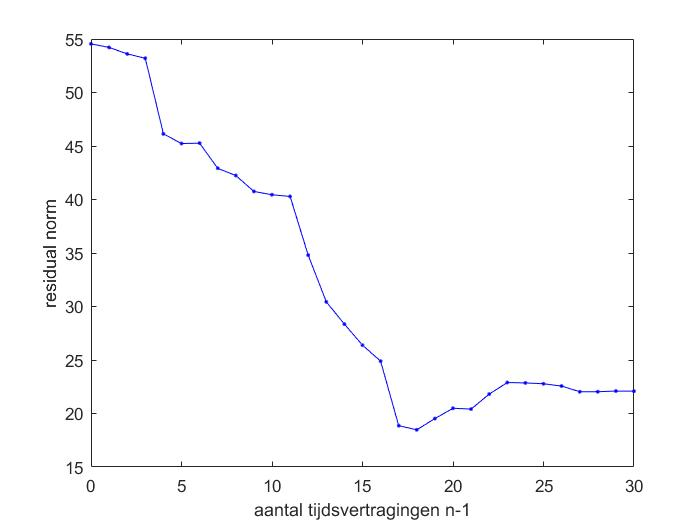
\includegraphics[width=0.7\textwidth]{oef3.jpg}
    \caption{Validatie van het model bij verschillende tijdsvertragingen}
    \label{fig:oef3}
\end{figure}